\documentclass[uplatex,dvipdfmx,a4paper,11pt]{jsarticle}

\usepackage{docmute}


% 数式
\usepackage{amsmath,amsthm,amssymb}
\usepackage{bm}
% 画像
\usepackage{graphicx}

\usepackage{multirow}
\usepackage{wrapfig}
\usepackage{ascmac}
\usepackage{xcolor}


\usepackage{makeidx}
\makeindex

\graphicspath{{../../_Figures//}{../../_Figures/Rheology/}}

\usepackage{qrcode}
\setlength\lineskiplimit{0pt}
\setlength\normallineskiplimit{0pt}

\usepackage{qexam}

\usepackage{titlesec}
\titleformat*{\section}{\Large\bfseries}
\titleformat*{\subsection}{\large\bfseries}
\titleformat*{\subsubsection}{\normalsize\bfseries}
\titleformat*{\paragraph}{\normalsize\bfseries}

% ページ設定
% \pagestyle{empty}
% 高さの設定
\setlength{\textheight}{\paperheight}   % ひとまず紙面を本文領域に
\setlength{\topmargin}{-5.4truemm}      % 上の余白を20mm(=1inch-5.4mm)に
\addtolength{\topmargin}{-\headheight}  % 
\addtolength{\topmargin}{-\headsep}     % ヘッダの分だけ本文領域を移動させる
\addtolength{\textheight}{-40truemm}    % 下の余白も20mmに%% 幅の設定
\setlength{\textwidth}{\paperwidth}     % ひとまず紙面を本文領域に
\setlength{\oddsidemargin}{-5.4truemm}  % 左の余白を20mm(=1inch-5.4mm)に
\setlength{\evensidemargin}{-5.4truemm} % 
\addtolength{\textwidth}{-40truemm}     % 右の余白も20mmに
% 図と本文との間
%\abovecaptionskip=-5pt
%\belowcaptionskip=-5pt
%
% 全体の行間調整
% \renewcommand{\baselinestretch}{1.0} 
% 図と表
%\renewcommand{\figurename}{Fig.}
%\renewcommand{\tablename}{Tab.}
%

% \makeatletter 
% \def\section{\@startsection {section}{1}{\z@}{1.5 ex plus 2ex minus -.2ex}{0.5 ex plus .2ex}{\large\bf}}
% \def\subsection{\@startsection{subsection}{2}{\z@}{0.2\Cvs \@plus.5\Cdp \@minus.2\Cdp}{0.1\Cvs \@plus.3\Cdp}{\reset@font\normalsize\bfseries}}
% \makeatother 

\usepackage[dvipdfmx,%
 bookmarks=true,%
 bookmarksnumbered=true,%
 colorlinks=false,%
 setpagesize=false,%
 pdftitle={数式に頼らない直感的理解による材料設計のためのレオロジー⼊⾨},%
 pdfauthor={佐々木裕},%
 pdfsubject={},%
 pdfkeywords={レオロジー; 材料設計; }]{hyperref}
\usepackage{pxjahyper}

\usepackage{plext}

\usepackage{niceframe} 
\usepackage{framed}
\newenvironment{longartdeco}{%
  \def\FrameCommand{\fboxsep=\FrameSep \artdecoframe}%
  \MakeFramed {\FrameRestore}}%
 {\endMakeFramed}
 
\usepackage{siunitx}

\newcommand{\rmd}{\mathrm{d}}

\usepackage[inline]{showlabels}

\begin{document}

\section*{この章の内容}

具体的なレオロジーの議論に入る前に、もう少しだけ、レオロジーに関する物理モデルを理解するために必要となる数学と物理の基礎的な事項について確認していきましょう。
ここでは、前章よりは少し難しい話になり、高校から大学レベルのお話をすることになります。

まず、レオロジーに関する物理モデルを作っていくときに必要となる2つの関数を説明し、続いて、その数学的な議論をすすめるための微分方程式を解けるように微分と積分という考え方について、そのイメージの部分だけを概観していきます。
また、その物理モデルを我々が取り扱いたい物質の物理へとつなげるために、力とポテンシャルの関係についても微積分を利用して理解を深めていきます。

具体的な事項を以下に列記しました。
\begin{boxnote}
	\large
	\begin{itemize}
		\item レオロジーで扱う関数について
		\begin{itemize}
			\item 指数関数と対数関数について
		\end{itemize}
		\item 微積分について
		\begin{itemize}
			\item 微積分について
			\item 簡単な微分方程式の解き方
		\end{itemize} 
		\item 物理モデルを物質の物理とつなげるために
		\begin{itemize}
			\item 力、仕事、ポテンシャルと微積分
			\item 摩擦と熱について
		\end{itemize} 
	\end{itemize}
\end{boxnote}

\section{レオロジーで扱う関数について}

\subsection{関数の一覧}

以前に、関数\index{かんすう@関数}について簡単に触れて、物理的なイメージを得るためには線型\index{せんけい@線型}性が成り立つような範囲で議論するとかんたんにモデル化できるということをお話しました。
これは関数としては、一次関数ということになります。
確かに、線型\index{せんけい@線型}関係に持ち込めれば単純化できて便利なのですが、事象の関係はそう単純に進むわけでもありません。

様々な関数\index{かんすう@関数}について、表 \ref{kansu} に一覧にまとめました。
何もここで、数学的に面倒なお話をするつもりはありませんが、これらの関数も当然使いみちがあり非常に有用なのです。
その位置づけを確認する意味で、少し違う観点で、初等関数というものを確認します。
実用的に簡単に言いきってしまえば、高校までの数学で習った範囲での関数ということになります。

\begin{itembox}[l]{Wikipedia での「初等関数」の説明}
	初等関数とは、\href{https://ja.wikipedia.org/wiki/%E5%88%9D%E7%AD%89%E9%96%A2%E6%95%B0#:~:text=%E5%88%9D%E7%AD%89%E9%96%A2%E6%95%B0%EF%BC%88%E3%81%97%E3%82%87%E3%81%A8%E3%81%86%E3%81%8B%E3%82%93%E3%81%99%E3%81%86,%E3%81%AA%E3%81%A9%E3%81%AF%E5%88%9D%E7%AD%89%E9%96%A2%E6%95%B0%E3%81%A7%E3%81%AA%E3%81%84%E3%80%82}{Wikipedia の「初等関数」} によれば、「実数または複素数の1変数関数で、代数関数、指数関数、対数関数、三角関数、逆三角関数および、それらの合成関数を作ることを有限回繰り返して得られる関数のことである。」と書かれています。

	% なお、\href{https://ja.wikipedia.org/wiki/%E9%96%A2%E6%95%B0_(%E6%95%B0%E5%AD%A6)}{Wikipedia の「関数(数学)」} の真ん中あたりに、多様な関数をクラス分けした見やすい表があります。
\end{itembox}

代数関数というのも本来の定義はちょっと面倒ですが、中学程度で習った多項式関数(一次関数、二次関数、等\footnote{
	その他に、分数関数、無理関数があります。
})をイメージしていただければいいと思います。

レオロジーを理解するために必要となる関数\index{かんすう@関数}としては、よく使われるものとして、指数関数\index{しすうかんすう@指数関数}と対数関数\index{たいすうかんすう@対数関数}を挙げることができます。
ここでは、その2つについて簡単に確認します。

\begin{table}[tb]
	\begin{center}
		\caption{様々な関数}
		\label{kansu}
		\begin{tabular}{|c|c|c|c|c|c|} \hline
			\multicolumn{5}{|c|}{関数} &	具体例 \\ \hline
			\multirow{11}{*}{ \pbox<t>{初等関数} } & \multirow{6}{*}{ \pbox<t>{代数関数} } & \multirow{5}{*}{ \pbox<t>{有理関数} } & \multirow{4}{*}{ \pbox<t>{多項式関数} }	&	定数関数	& $f(x) = a$	\\ \cline{5-6}
			&&&& 一次関数	& $f(x) = ax + b$	\\ \cline{5-6}
			&&&& 二次関数	& $f(x) = ax^2 + bx + c$ \\ \cline{5-6}
			&&&& 三次関数	& $f(x) = ax^3 + bx^2 + cx + d$	\\ \cline{4-6}
			&&& \multicolumn{2}{c|}{分数関数}	& $f(x) = \dfrac{a}{x}$	\\ \cline{3-6}
			&& \multicolumn{3}{c|}{無理関数}	& $f(x) = \sqrt{x}$	\\ \cline{2-6}
			& \multirow{5}{*}{ \pbox<t>{初等超越関数} } & \multicolumn{3}{c|}{指数関数}	& $f(x) = e^x$	\\ \cline{3-6}
			&& \multicolumn{3}{c|}{対数関数}	& $f(x) = \ln (x)$	\\ \cline{3-6}
			&& \multicolumn{3}{c|}{三角関数}	& $f(x) = \sin x$	\\ \cline{3-6}
			&& \multicolumn{3}{c|}{双曲線関数}	& $f(x) = \sinh x$	\\ \cline{3-6}
			&& \multicolumn{3}{c|}{冪関数}	& $f(x) = x^a$	\\ \hline
			\multirow{4}{*}{ \pbox<t>{特殊関数} } & \multicolumn{4}{c|}{ガンマ関数}	& $\Gamma (x)$	\\ \cline{2-6}
			& \multicolumn{4}{c|}{ベータ関数}	& B$(x,y)$	\\ \cline{2-6}
			& \multicolumn{4}{c|}{誤差関数}	& $erf(x)$	\\ \cline{2-6}
			& \multicolumn{4}{c|}{デルタ関数}	& $\Delta$	\\ \hline
		\end{tabular}
	\end{center}
\end{table}


\subsection{指数関数\index{しすうかんすう@指数関数}について}

\subsubsection{指数関数の定義}
指数関数\index{しすうかんすう@指数関数}を天下りに定義すると、「指数関数とは、冪における指数\index{しすう@指数}を変数として、その定義域を主に実数の全体へ拡張して定義される初等超越関数の一種である。」というように書かれています。
このような定義だけもみても具体的なイメージがわかりにくいので、まず、キーワードとして「冪(ベキとよみます。)」と、累乗の説明も合わせて示しました。
\large
\begin{itembox}[l]{「指数関数」の天下りな定義}
	「指数関数とは、冪における指数\index{しすう@指数}を変数として、その定義域を主に実数の全体へ拡張して定義される初等超越関数の一種である。」
	\begin{align*}
		f(x) = a^x
	\end{align*}
	\begin{itemize}
		\item 冪とは
		\begin{itemize}
			\item 「底」と呼ばれる正の数の右肩に「指数」と呼ばれる数を載せた数式表現であり、指数\index{しすう@指数}が自然数の場合に累乗と呼ばれる。
		\end{itemize}
		\item 累乗
		\begin{itemize}
			\item 「累」= 重ねる、「乗」= 掛ける\\
			したがって、累乗は複数回掛け合わせるということを意味します。
		\end{itemize}
		\begin{equation*}
			\underbrace{a\times a\times a \cdots \times a}_{\text{$n$個}} = a^n
		\end{equation*}
	\end{itemize}
\end{itembox}
\normalsize

\subsubsection{指数\index{しすう@指数}の性質}
指数\index{しすう@指数}の性質を簡単にまとめると以下のようになります。
\large
\begin{itembox}[l]{指数\index{しすう@指数}の性質}
	\begin{itemize}
		\item 累乗同士の掛け算は、指数同士の足し算 $a^n \times a^m = a^{(n+m)}$
		\item 累乗のさらなる累乗は、指数同士の掛け算 $(a^n)^m = a^{(n \times m)}$
		\item 指数が 0 の場合は? $a^0 = 1$
		\item 指数が負 $\Rightarrow$ 指数が正の逆数 $a^{-k} = \dfrac{1}{a^k}$
		\item 指数同士の割り算は指数の引き算 $a^n \div a^m = a^{n-m}$
		\item 指数が分数の場合
			\begin{itemize}
				\item 分数の分母となる値を用いて累乗根を表し、
				\item 分子はそのべき乗を表す\\
				$a^{\frac{m}{n}}=\sqrt[n]{a^m}$
			\end{itemize}
	\end{itemize}
\end{itembox}
\normalsize
上記のような性質を天下りに暗記してもいいのですが、指数\index{しすう@指数}が自然数だけで定義される「累乗としての性質」を確認した上で、その声質をベースとして、指数\index{しすう@指数}を整数、そして、有理数へと拡張して、性質の由来を確認していきましょう。

このように、限定的な条件で成立した性質を基礎として、条件をより広い範囲へと広げてその声質を確認していくような考え方は、物理モデル\index{ぶつりもでる@物理モデル}を考えるときにも非常に役に立ちます。
できれば、自分の手を動かして確認してみてください。

\paragraph{指数\index{しすう@指数}が自然数の場合}
まず、指数\index{しすう@指数}が自然数の場合に限定して、議論しましょう。

同じ底の累乗同士の掛け算は、
\begin{align*}
a^n \times a^m 	&= (\underbrace{a\times a\times a \cdots \times a}_{\text{$n$個}}) \times (\underbrace{a\times a\times a \cdots \times a}_{\text{$m$個}}) \notag \\
		&= \underbrace{a\times a\times a \cdots \times a}_{\text{$n+m$個}} \notag \\
		&= a^{(n+m)}
\end{align*}
となり、指数同士の足し算となります。

また、累乗のさらなる累乗は、
\begin{align*}
(a^n)^m 	&= \underbrace{(\underbrace{a\times a \cdots \times a}_{\text{$n$個}}) \times (\underbrace{a\times a \cdots \times a}_{\text{$n$個}}) \cdots \times (\underbrace{a\times a \cdots \times a}_{\text{$n$個}})}_{\text{$m$}個} \notag \\
		&= \underbrace{a\times a\times a \cdots \times a}_{\text{$n \times m$個}} \notag \\
		&= a^{(n \times m)}
\end{align*}
この場合は、指数\index{しすう@指数}同士の掛け算となります。

さらに、異なる底の累乗同士の掛け算は指数\index{しすう@指数}が同一の場合にだけ可能であり、
\begin{align*}
a^n \times b^n 	&= (\underbrace{a\times a\times a \cdots \times a}_{\text{$n$個}}) \times (\underbrace{b\times b\times b \cdots \times b}_{\text{$n$個}}) \notag \\
		&= \underbrace{(a \times b) \times (a \times b) \cdots \times (a \times b)}_{\text{$n$個}} \notag \\
		&= (a \times b)^n
\end{align*}
というように底同士の掛け算としてまとめることができます。

指数\index{しすう@指数}が自然数であった場合の、累乗に関する公式は以上の三つとなります。

\paragraph{整数への拡張}
これから、指数の定義域を拡張して行きましょう。
これ以降の拡張は、上記の基本となる累乗の三つの公式を満たすように拡張して行くことになります。

指数の定義域を整数へと拡張するために、最初に、$a \ne 0(a^n\ne0)$ としておいて、指数が0の場合($a^0$)を考えましょう。
累乗同士の掛け算の関係式を用いると、
\begin{align*}
a^n \times a^0 =a^{(n+0)} = a^n 
\end{align*}
$a^n \ne 0$であるので、上式の両辺を$a^n$で除して、
\begin{equation*}
a^0 = 1
\end{equation*}
が得られます。

これを、指数が0の場合($a^0$)の定義として表現すると、「$a \ne 0$ である任意の実数 $a$ について,$a^0 = 1$ が成り立つ」とということになります
\footnote{
なお、$a = 0$ のときは、$0^0$ は不定となるため、考えないこととします。
}。

さらに、負の数への拡張として、$k$ が正の整数だった場合の、$a^{-k}$ について考えてみましょう。
\begin{equation*}
a^k \times a^{-k} = a^{k+(-k)}=a^0=1
\end{equation*}
最後の変換で、上記の指数が 0 の定義を用いています。
そして、$a^k$ で両辺を除すと、
\begin{equation*}
a^{-k} = \dfrac{1}{a^k}
\end{equation*}
結局、指数が負の場合は、指数が正であった場合の逆数となるように定義することができます。

このとき、指数同士の割り算を考えれば、以下のように指数の引き算となります。
\begin{equation*}
a^n \div a^m =a^n \times \dfrac{1}{a^m} = a^n \times a^{-m} = a^{n + (-m)}
\end{equation*}

\paragraph{有理数への拡張}
最後に、分数(有理数)にまで拡張しましょう。
この拡張は、特別なことを定義する必要もなく、指数が分数の場合においても、これまでに示してきたような指数の公式に基づいて計算を行うということになります。

指数が分数の場合として、$a^{m/n}$(ただし、$n$、$m$は整数)というものを考えると、この累乗は、
\begin{equation*}
(a^{\frac{m}{n}})^n=a^{\frac{m}{n} \times n}=a^m
\end{equation*}
すなわち、$a^{m/n}$ の $n$ 乗が $a^m$ となると考えることができます。

ここで、一般には、実数 $x$ に対して $x$ を $n$ 乗すると $y$ になるとき($n$ は正の整数)、$y$ を「$x$ の $n$ 乗根」と呼び、$\sqrt[n]{x}$ と表記するのでした。

この関係を用いると、上記の指数が分数の場合は、指数となる分数の分母となる値を用いて累乗根を表し、以下のように記述できることになります。
\begin{equation*}
a^{\frac{m}{n}}=\sqrt[n]{a^m}
\end{equation*}

\paragraph{指数関数\index{しすうかんすう@指数関数}の特徴}
独立変数として実数である $x$ を指数とする関数を、一般に指数関数と呼びます。
\begin{equation*}
f(x)=a^x
\end{equation*}

$y=a^x$としたとき、 $xy$平面上でのグラフは以下の特徴を持っています。

物理的な議論においては、底としてネイピア数$e$を用いる場合が非常に多くなります
\footnote{ネイピア数$e$は、$\pi$と同様に多用される数学定数の一つであり、その値は、$e=2.718281828 \cdots $と続く「超越数」です。}。
ここでは、底が $e$ の場合を、独立変数を見やすくするために、$\exp (x)$ と表記します。
\begin{figure}[htb]
	\begin{center}
		\begin{minipage}{0.45\textwidth}
			\large
			\begin{itembox}[l]{指数関数の特徴}
				\begin{itemize}
					\item \textcolor{red}{$\exp (x)$ は、単調増加。}
					\item \textcolor{green}{$\exp (-x) = \left(\dfrac{1}{e} \right)^x$ は、\\単調減少。}
					\item 常に、点$(0,1)$を通る。
					\item $x$軸($y=0$)を漸近線
				\end{itemize}
			\end{itembox}
		\end{minipage}
		\begin{minipage}{0.45\textwidth}
			\begin{center}
			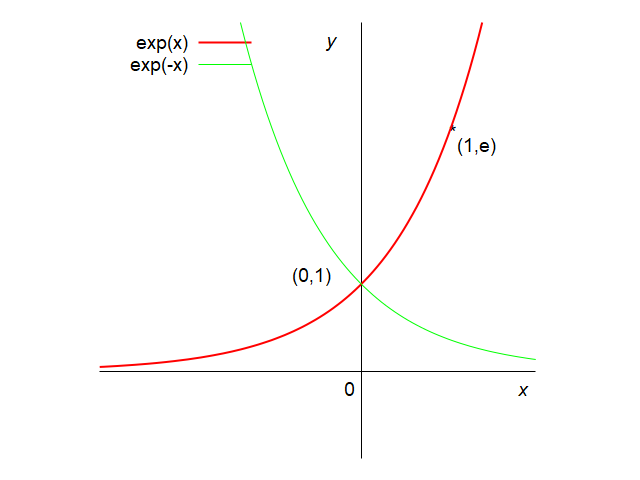
\includegraphics[width=\textwidth]{exp.png}
			\end{center}
		\end{minipage}
		\caption{指数関数の特徴}
		\label{fig: exp(x)}
	\end{center}
\end{figure}

指数関数 $y = \exp (x)$ のグラフを、図 \ref{fig: exp(x)} に示しました。
$x=0$ において $y=1$ であり、$x$ の増加に伴い単調増加し、$x=1$ では $y=e$ となっています。
指数が負である場合は単調減少となるが、いずれの場合も、関数の値は正となります。

\subsection{対数関数\index{たいすうかんすう@対数関数}について}

\subsubsection{対数関数とは}
対数関数\index{たいすうかんすう@対数関数}とは、指数関数\index{しすうかんすう@指数関数}とは表裏一体であり、逆関数となっています。
この関係を、図 \ref{shisuu_taisuu} に示しました。
\begin{figure}[htb]
	\begin{center}
		\begin{minipage}{0.45\textwidth}
			\large
			\begin{itembox}[l]{指数関数と対数関数}
				\vspace{-3mm}
				\begin{align*}
					\textcolor{blue}{a}^{\textcolor{red}{x}} = \textcolor{green}{M} \Leftrightarrow \textcolor{red}{x}= \log_{\textcolor{blue}{a}} \textcolor{green}{M}
				\end{align*}
				\begin{itemize}
					\item 指数関数:底に指数を作用させて真数を求める関数
					\item 対数関数:真数は底にどんな指数を与えたものかを求める関数
					\item $y = x$ のグラフに関して対称
				\end{itemize}
			\end{itembox}
		\end{minipage}
		\begin{minipage}{0.45\textwidth}
			\begin{center}
			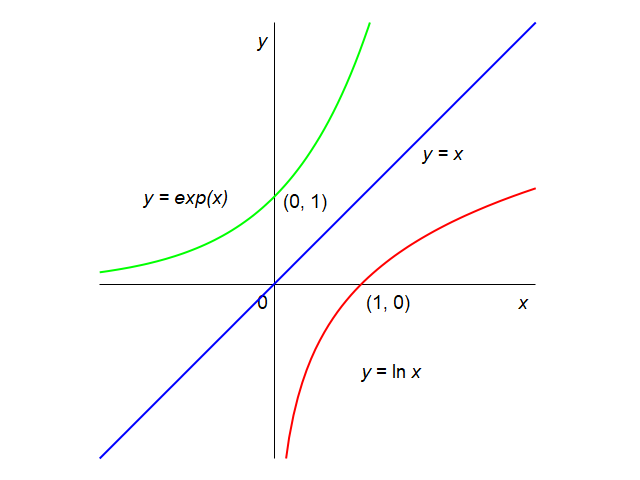
\includegraphics[width=\textwidth]{exp_ln.png}
			\end{center}
		\end{minipage}
		\caption{指数関数と対数関数の関係}
		\label{shisuu_taisuu}
	\end{center}
\end{figure}

\subsubsection{対数\index{たいすう@対数}の性質}
対数関数\index{たいすうかんすう@対数関数}の性質を以下にまとめました。
これらの性質は、指数関数のものと同様に導出できますので、ここでは一覧として示すだけにします。
一度自分の手を動かして導出されることをお勧めします。
\large
\begin{itembox}[l]{対数関数の性質}
	任意の正の実数である $M,N$ に対して、
			\begin{itemize}
				\item 対数同士の足し算は、真数の掛け算 $\ln (M \times N) = \ln M + \ln N$
				\item 対数同士の引き算は、真数の割り算 $\ln(M \div N) = \ln M - \ln N$
				\item 真数の冪は、冪を掛け算に $\ln M^p = p \ln M$
				\item 真数の逆数は、マイナスを付けて $\ln \dfrac{1}{M} = -\ln M$
				\item $\ln 1 = 0$
			\end{itemize}
\end{itembox}
\normalsize
対数関数は、大きな数を桁数でざっくりと見るときに便利であるという特徴があり、線弾性スペクトルのように極端に範囲の広いデータを取り扱うときに使用されます。

\subsubsection{対数\index{たいすう@対数}グラフ}
対数\index{たいすう@対数}のもう一つの有用な使いみちとして、グラフにおける軸を対数表示するという対数グラフというものがあり、一つの軸のみを対数表示した「片対数グラフ\index{かたたいすう@片対数グラフ}」と、両方の軸を対数化した「両対数グラフ\index{りょうたいすう@両対数グラフ}」があります。

\paragraph{片対数\index{かたたいすう@片対数}グラフ}
片対数グラフ\index{かたたいすう@片対数グラフ}とは、一つの軸のみを対数表示したものとなります。

指数関数で表される数式があったとき、両辺の対数\index{たいすう@対数}を取ると、以下のように展開できます。
\begin{align*}
	y&=\exp(ax+b) \\
	\therefore \; \ln y &= ax + b
\end{align*}

このとき、縦軸を対数目盛としたグラフにプロットすれば、その傾きが $a$、$y$ 切片が $b$ となる直線が得られるわけです。

\begin{figure}[htb]
	\begin{center}
		\begin{minipage}{0.45\textwidth}
			\large
			\begin{itembox}[l]{片対数グラフの例}
				\begin{itemize}
					\item 指数関数を取り扱う際に、
					\item 両辺の対数を取ると、\\
					$\ln y = ax + b$
					\begin{itemize}
						\item 関数値の対数が、
						\item 変数の1次関数となる。
						\item 指数が傾きとして求まる。
					\end{itemize}
				\end{itemize}
			\end{itembox}
		\end{minipage}
		\begin{minipage}{0.45\textwidth}
			\begin{center}
			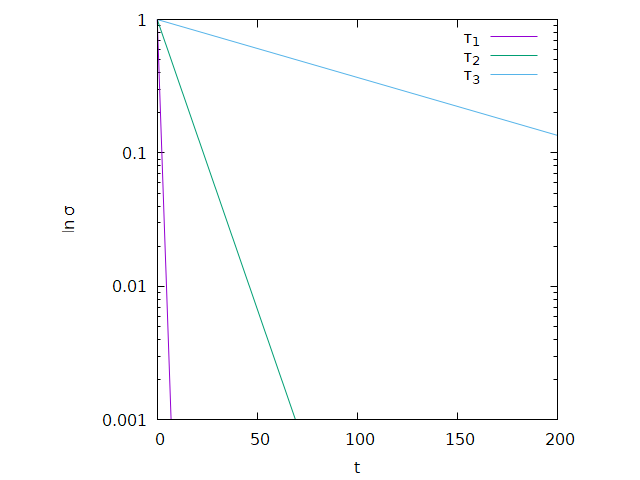
\includegraphics[width=\textwidth]{relux_6.png}
			\end{center}
		\end{minipage}
		\caption{片対数グラフの例}
		\label{fig:semilog}
	\end{center}
\end{figure}

\paragraph{両対数\index{りょうたいすう@両対数}グラフ}
両対数グラフ\index{りょうたいすう@両対数グラフ}とは、両方の軸を対数で表示したものです。
\begin{figure}[htb]
	\begin{center}
		\large
		\begin{minipage}{0.45\textwidth}
			\begin{itembox}[l]{両対数グラフの意味}
				\begin{itemize}
					\item 極端に範囲の広いデータを扱えるため、粘弾性スペクトルは、通常この形で表される。
					\item 冪関数 $y = x^a$ を線型で処理できる。
					\begin{align*}
						\log y = a \log x
					\end{align*}
					両対数グラフにプロットすれば、その傾きが決まる。
				\end{itemize}
			\end{itembox}
		\end{minipage}
		\begin{minipage}{0.45\textwidth}
			\begin{center}
			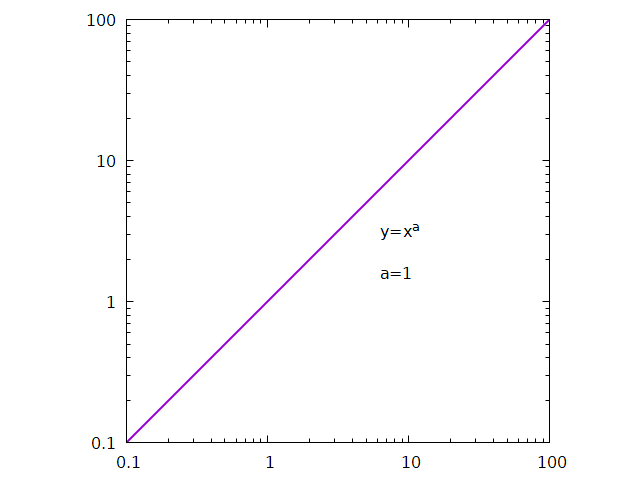
\includegraphics[width=\textwidth]{beki.png}
			\end{center}
		\end{minipage}
		\caption{両対数グラフの例}
		\label{fig:loglog}
	\end{center}
\end{figure}

\section{微積分\index{びせきぶん@微積分}について}

\subsection{微分\index{びぶん@微分}について}
微分とは、「対象とする関数\index{かんすう@関数}が、注目したい点の周りでどのように振る舞うのかを、明らかにする方法」と考えることができます。

\subsubsection{微分\index{びぶん@微分}の考え方}
微分の直感的なイメージとしては、注目する点における関数の振る舞いを接線の傾きで表したものと考えることができます。
\begin{figure}[htb]
	\begin{center}
		\begin{minipage}{0.5\textwidth}
			\large
			\begin{itembox}[l]{微分の直感的説明}
				\begin{itemize}
					\item 注目する点近傍での、接線の「傾き」
					\begin{itemize}
						\item 変数の増分と、
						\item 関数の増分との比
					\end{itemize}
					\item 変数の増分を無限小にしたとき、
				\end{itemize}
			\end{itembox}
		\end{minipage}
		\begin{minipage}{0.4\textwidth}
			\begin{center}
			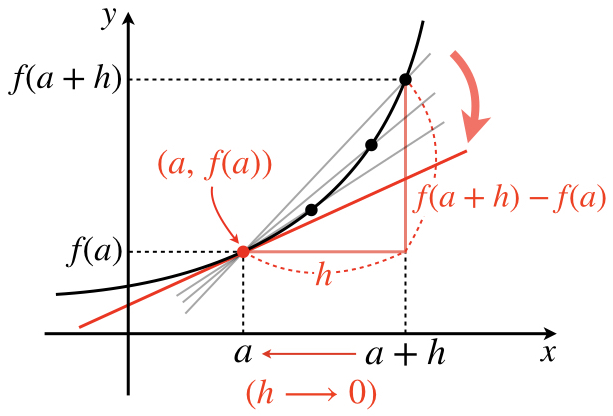
\includegraphics[width=\textwidth]{bibun.jpeg}
			\end{center}
		\end{minipage}
		\caption{微分の考え方}
		\label{bibun}
	\end{center}
\end{figure}

関数 $f(x)$ を $x$ で微分することを、$\dfrac{\mathrm{d} f(x)}{\mathrm{d}x}$ と書き表します。
ここでの、d が微小量の変化であることを表し、「分母である変数」と「分子となっている関数」との「僅かな変化の比」をとるイメージとなっています。

\large
	\begin{itembox}[l]{微小な変化の比}
		\begin{itemize}
			\item 関数 $f(x)$ を $x$ で微分することを、
			\item $\dfrac{\mathrm{d} f(x)}{\mathrm{d}x}=\dfrac{\text{関数の微小変化量}}{変数の微小変化量}$ 
			\begin{itemize}
				\item ``d'' が微小量の変化であることを表し、
				\item 「分母である変数」と「分子となっている関数」との「僅かな変化の比」
			\end{itemize}
		\end{itemize}
	\end{itembox}
\normalsize

\subsubsection{微分のイメージ}
もう少しだけ、直感的な理解につながるアナロジーを考えていきましょう。

自転車の発電式(ダイナモ)ライトを例に取ってみます。

\begin{figure}[htb]
	\begin{center}
		\begin{minipage}{0.5\textwidth}
			\large
			\begin{itembox}[l]{自転車のライトの例}
				\begin{itemize}
					\item 速度を上げると明るく、止まると\\消える。
					\begin{itemize}
						\item 明るさが瞬間的な速度
						\item 微分の値の大小に対応
					\end{itemize}
					\item 明るさ $\Leftrightarrow$ 非常に短い時間あたりに\\進める距離
				\end{itemize}
			\end{itembox}
		\end{minipage}
		\begin{minipage}{0.4\textwidth}
			\begin{center}
			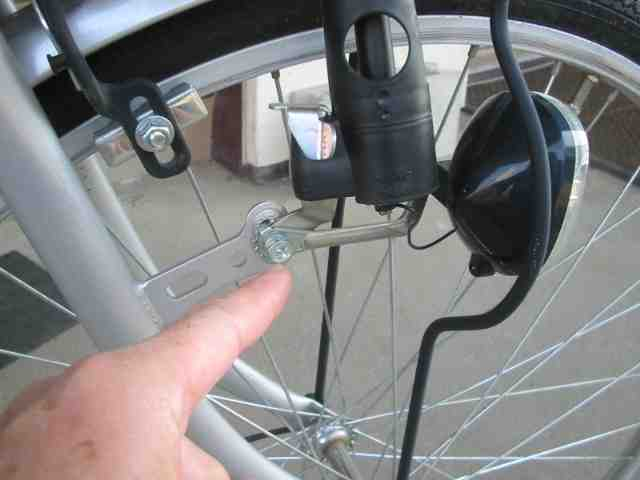
\includegraphics[width=.8\textwidth]{bike.jpg}
			\end{center}
		\end{minipage}
		\caption{自転車のライトの例}
		\label{bike_light}
	\end{center}
\end{figure}

このアナロジーからも、微分で見ることで関数の瞬間的な振る舞いを見ることができるとわかります。
\begin{itemize}
	\item 微分大 $\Leftrightarrow$ その瞬間に変化量が大きい
	\item 微分小 $\Leftrightarrow$ その瞬間にはあまり変化しない。
\end{itemize}

\subsubsection{微分\index{びぶん@微分}の公式}
微分の公式には様々なものがありますが、今回の講座として取り扱う微分に関する公式は、表 \ref{bibun_kousiki} に示したようなものぐらいです。

\renewcommand{\arraystretch}{2}
\begin{table}[tb]
	\begin{center}
		\caption{微分の公式}
		\label{bibun_kousiki}
			\begin{tabular}{|c|c|c|} \hline
				微分の対象		& 公式							& メモ \\ \hline \hline
				冪の微分		& $\dfrac{\mathrm{d}}{\mathrm{d}x}x^a = ax^{a-1}$ 		&  多項式では線形性も利用\\ \hline
				指数関数の微分	& $\dfrac{\mathrm{d}}{\mathrm{d}x}\exp(x) = \exp(x)$ 		&  ネイピア数の場合\\ \hline
				自然対数の微分	& $\dfrac{\mathrm{d}}{\mathrm{d}x}\ln x = \dfrac{1}{x}$ 	& 底がネイピア数 \\ \hline
			\end{tabular}
		\end{center}
\end{table}
\renewcommand{\arraystretch}{1.}

\subsection{積分\index{せきぶん@積分}について}
積分には、大きく分けて2つの使い方があります。
一つは、定積分と呼ばれる、処理する範囲を定めて計算するやり方であり、イメージとしては関数が占める範囲を面積として表すような考え方ということになり、もう一つは、不定積分と呼ばれる処理の範囲を定めることなく数式の変換を行うものであり、微分\index{びぶん@微分}の逆変換というイメージで捉えることができます。

\subsubsection{定積分\index{ていせきぶん@定積分}について}
まず、定積分についての説明から始めます。

定積分が表すものは、直感的には、指定した範囲における、関数 $f(x)$ が表す曲線と $x$ 軸との間の「面積」と考えることができます。
この面積を求めるために、変数の微小な刻み $\mathrm{d} x$ と、その点近傍での関数 $f(x)$ との積 $f(x) \mathrm{dx}$(これは、グラフの短冊の部分の面積にあたります)を指定した範囲に渡って積算することになります。
\begin{figure}[htb]
	\begin{center}
		\begin{minipage}{0.45\textwidth}
			\large
			\begin{itembox}[l]{定積分の考え方}
				\begin{itemize}
					\item 直感的には「面積」
					\begin{itemize}
						\item \textcolor{green}{微小な刻み $\mathrm{d} x$} と
						\item \textcolor{red}{$f(x)$} との積(面積:\\グラフの短冊)を
						\item \textcolor{blue}{積算}する。
					\end{itemize}
					\vspace{-3mm}
					\small
					\begin{align*}
						\left[ F(x) \right]_a^b = \textcolor{blue}{\int_a^b} \textcolor{red}{f(x)} \textcolor{green}{\mathrm{d} x}
					\end{align*}
				\end{itemize}
			\end{itembox}
		\end{minipage}
		\begin{minipage}{0.45\textwidth}
			\begin{center}
			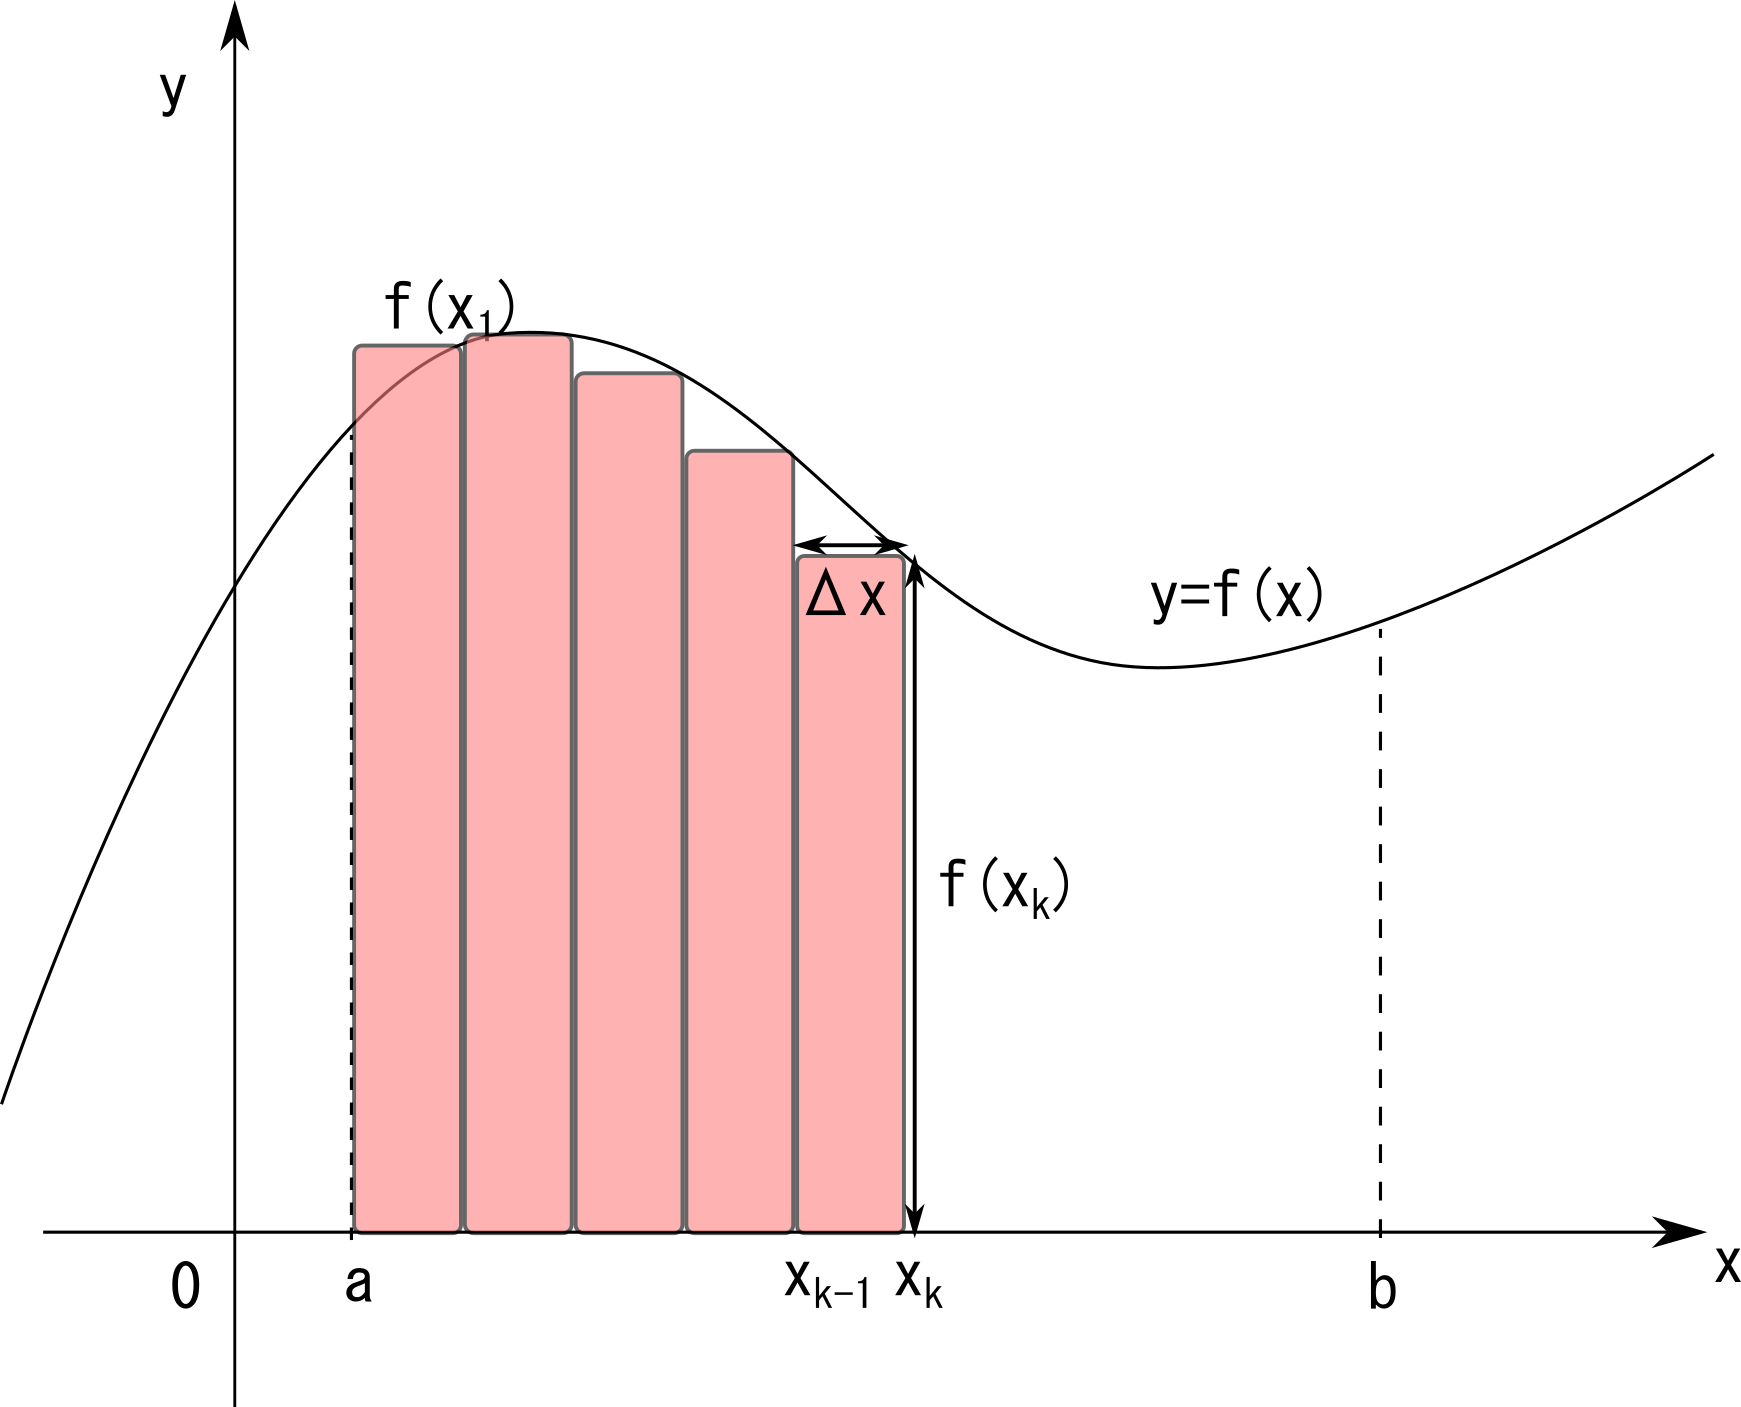
\includegraphics[width=.8\textwidth]{integral.png}
			\end{center}
		\end{minipage}
		\caption{定積分のイメージ}
		\label{sekibun}
	\end{center}
\end{figure}

この積算するということを、和(Summation)を表すギリシア記号 $\sum$ から、その頭文字の ``S'' を流用して縦方向に長く伸ばしたものである、インテグラル $\int$ という積分記号で表しているのです。そして、どの範囲を積分するのかということを積分記号の上と下に示します。
\large
\begin{itembox}[l]{自動車の移動の例}
	\begin{itemize}
		\item 速度が時間 $t$ の関数として $v(t)$ で表されるとき、
		\item 時刻 $t_0$ から $t_1$ までに進んだ距離 $L$ は、
	\end{itemize} 
	\begin{align*}
		L=\int_{t_0}^{t_1} v(t) \mathrm{d} t
	\end{align*}
\end{itembox}
\normalsize

\subsubsection{不定積分\index{ふていせきぶん@不定積分}について}
つぎに、不定積分として、微分の逆変換を行うことについての説明に進みます。

不定積分とは、積分範囲を定めない(不定)積分処理を行うことにより、微分するとその関数 $f(x)$ に一致するような関数(原始関数と呼ばれます)$F(x)$ を求める操作ということができます。
したがって、積分を微分の逆操作だととして考えると、不定積分により求めた式の両辺を微分すれば、元の関数が出てくることになるわけです。

なお、この処理において、定数 $C$ (積分定数)の分だけ不定値が出ることになります。

\large
\begin{itembox}[l]{微分の逆操作としての不定積分}
	\begin{itemize}
		\item 微分するとその関数 $f(x)$ に一致するような
		\item 原始関数 $F(x)$ を求める操作
		\begin{itemize}
			\item 積分範囲を定めない(不定)
			\item このとき、定数 $C$ (積分定数)だけ不定値が出る。
		\end{itemize}
			\begin{align*}
				F(x) = \int f(x) \mathrm{d} x +C
			\end{align*}
		\item (逆操作)両辺を微分すれば、元の関数
			\begin{align*}
				\dfrac{\mathrm{d}}{\mathrm{d} x} F(x) = f(x)
			\end{align*}
	\end{itemize}
\end{itembox}
\normalsize

\subsection{微積分\index{びせきぶん@微積分}とは}

では、微積分\index{せきぶん@積分}を使うことの意味について考えていきます。

微分を使うことで、任意の瞬間における関数の振る舞いの描像を取り出すことができます。
そして、積分を行うことで、注目する範囲全体に渡る関数の振る舞いの結果を総量として把握できるようになるのです。

\large
	\begin{itembox}[l]{微積分を使うこととは?}
		\begin{itemize}
			\item 微分で瞬間の描像を取り出し、
			\item 積分で全体のふるまいを総量として把握。
		\end{itemize}
	\end{itembox}
\normalsize

別の観点で考えると、小学校の算数においては、物事の変化が一定の値に従って(平均値で)生じていると考えて、単純に割り算や掛け算で処理していたわけです。
しかしながら、実際の振る舞いは瞬間ごとに異なる場合が多いので、単純な計算では対処できなくなります。
そのときに、微分や積分の出番となるわけです。
\begin{figure}[htb]
	\begin{center}
		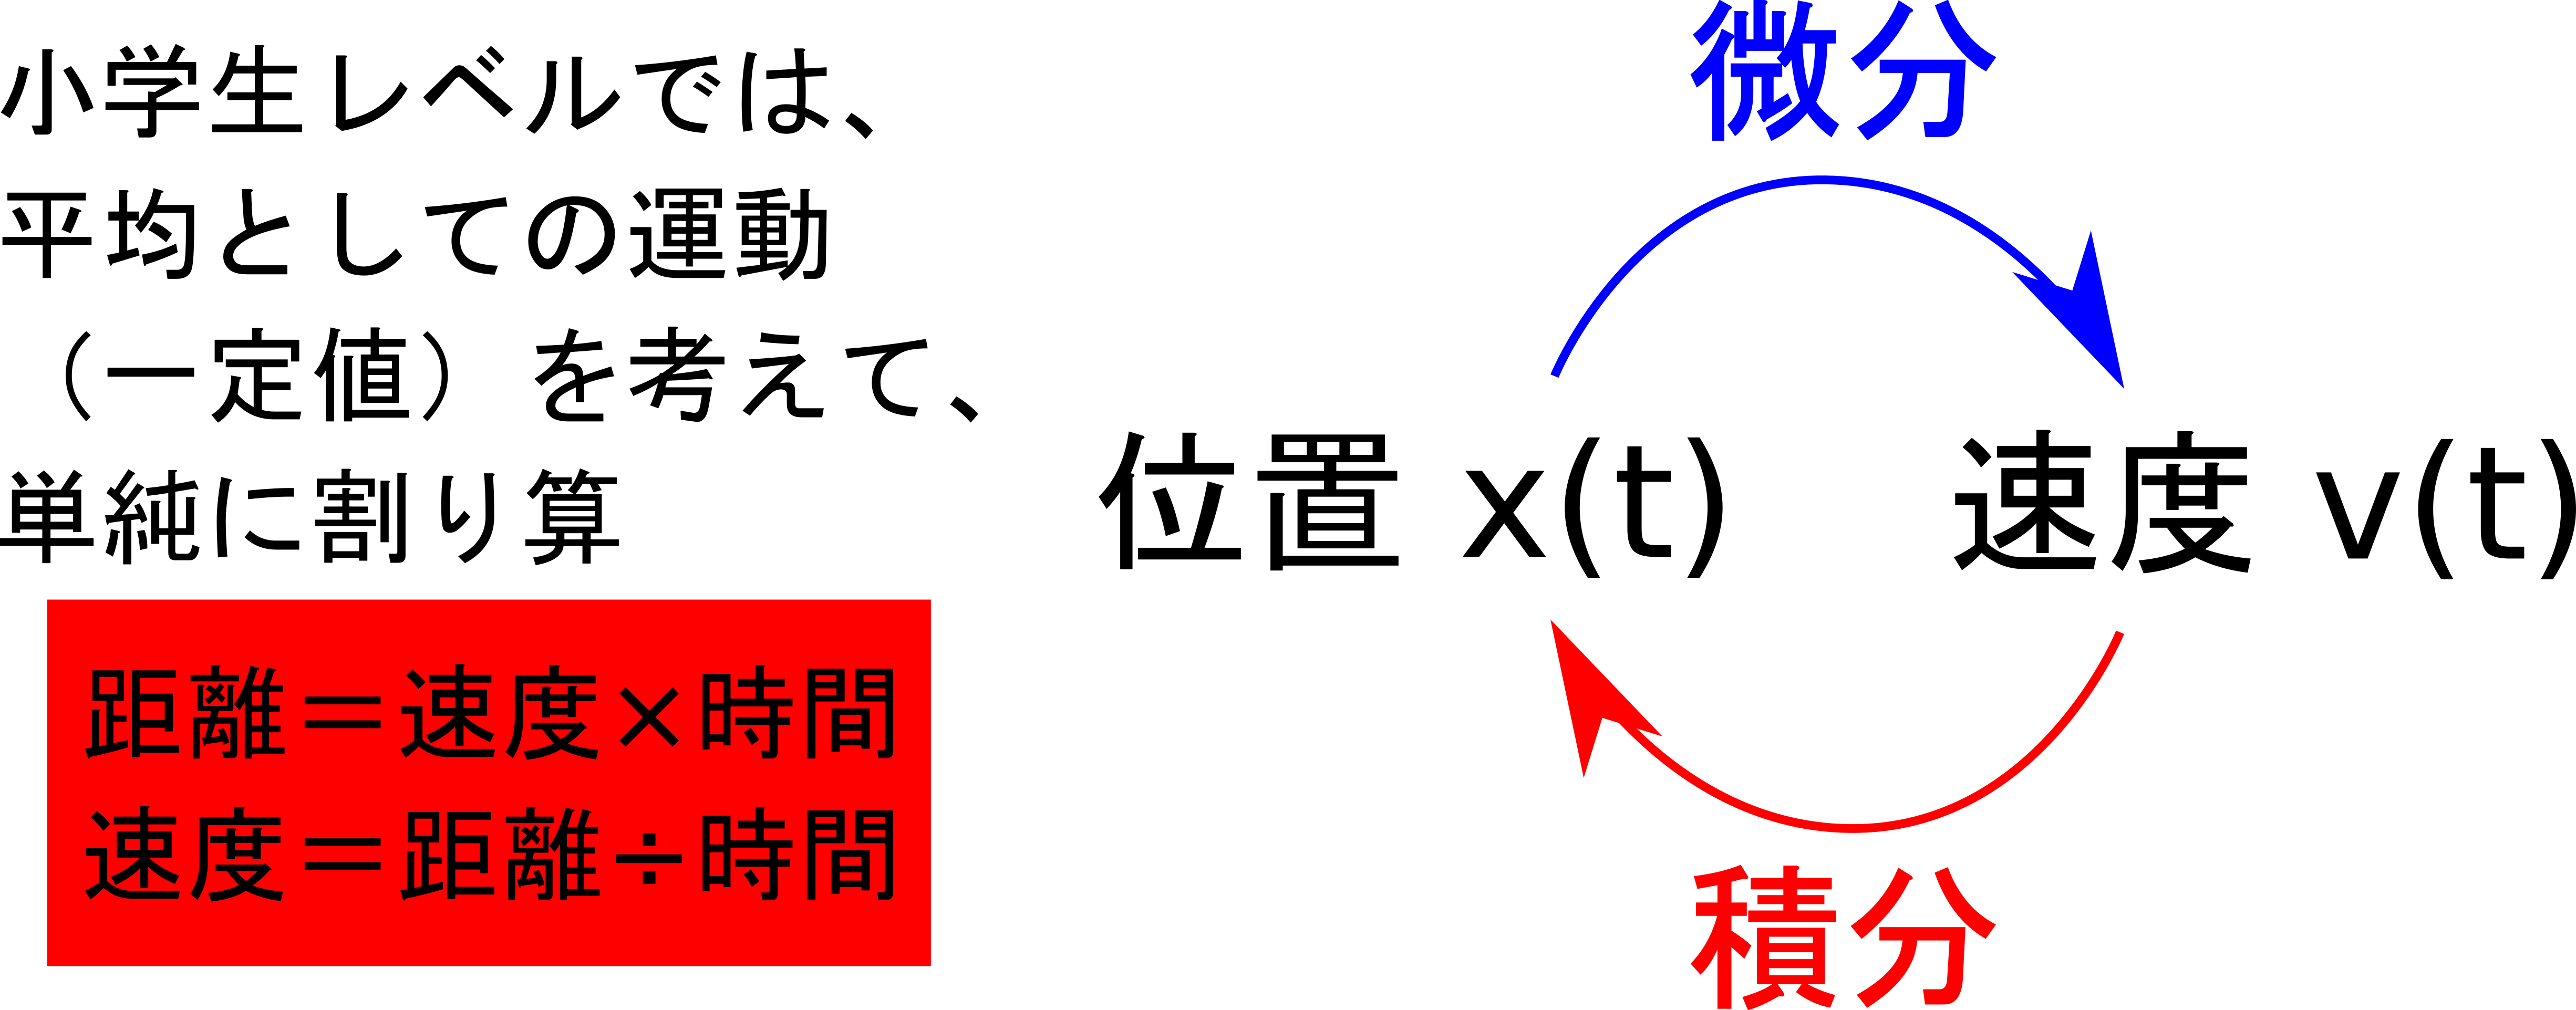
\includegraphics[width=.8\textwidth]{biseki.png}
		\caption{微分と積分の関係}
		\label{fig:biseki}
	\end{center}
\end{figure}

\subsection{簡単な微分方程式\index{びぶんほうていしき@微分方程式}}
やっと、微積分に関する準備が整いましたので、「物理モデル\index{ぶつりもでる@物理モデル}」を数学的に記述する際に必要となる「微分方程式」というものにお話を進めます。

\subsubsection{微分方程式\index{びぶんほうていしき@微分方程式}とは}
微分方程式とは、「物理現象や化学現象を、微分の形で記述したもの」であり、微分の逆操作である積分を用いることで解くことができます。
これを使いこなすことで、注目する現象の振る舞いをわかりやすい関数で表すことができるようになるわけです。
\large
	\begin{itembox}[l]{微分方程式とは?}
		「物理現象や化学現象を、微分の形で記述したもの」
			\begin{itemize}
				\item 例えば、「放射性物質の崩壊」等の、一次反応と呼ばれる化学現象を記述する頻出の微分方程式の形
				\begin{align*}
					\textcolor{red}{\dfrac{\mathrm{d}}{\mathrm{d} t} N(t)} = \textcolor{blue}{-aN(t)}
				\end{align*}
				\item この式の意味は、
				\begin{itemize}
					\item 左辺は\textcolor{red}{時間の関数である $N(t)$ の時間変化を微分の形}、
					\item 右辺はその変化が、\textcolor{blue}{$N(t)$ の量に比例して減少(負号がついているから)}することを表す。
					\item 定数 $a$ は [1/T] の次元を持つ。
				\end{itemize}
				\item \textbf{「積分\index{せきぶん@積分}を使って、方程式を解く。」}
			\end{itemize}
	\end{itembox}
\normalsize

\subsubsection{簡単な微分方程式の解き方の例}
微分方程式の解き方として、「変数分離」というものがあります。
これは、微分方程式の中で用いられている変数を、それぞれ、一方の辺に集めてしまうことを意味しています。
そして、微分量である $\mathrm{d}y$ や、$\mathrm{d}t$ を、演算可能な量を表すものとして扱います。

この解き方を用いて、上述の一次反応を表す微分方程式を実際に説いてみましょう。
\large
	\begin{itembox}[l]{一次反応を表す微分方程式を解いてみましょう}
		\textbf{1st step: }方程式の両辺に $\rmd t$ を掛ける。
		\begin{align*}
			\dfrac{1}{N} \mathrm{d}N= -a\mathrm{d} t
		\end{align*}

		\textbf{2nd step: }方程式の両辺に積分記号 $\int$ をつける。
		\begin{align*}
			\int \dfrac{1}{N} \rmd N = -a \int \mathrm{d} t
		\end{align*}

		\textbf{3rd step: }両辺の不定積分\index{ふていせきぶん@不定積分}を計算する。
		\begin{align*}
			\ln N +C_1 = -at + C_2
		\end{align*}

		\textbf{4th step: }積分定数を一つ($C=C_2-C_1$)にまとめる。
		\begin{align*}
			\ln N = -at + C
		\end{align*}

		\textbf{5th step: }指数関数\index{しすうかんすう@指数関数}に書き直してから、指数の性質を使って定数項を書き直し($C'=\exp(C)$)。
		\begin{align*}
			N=\exp(-at + C) = \exp(C) \times \exp(-at) = C' \exp(-at)
		\end{align*}

		これで、微分方程式としては一旦解けたことになるが、初期条件を考慮すれば定数項を定めることができる。
		$t=0$ での初期濃度が $N_0$ とすると、$\exp(-a*0) = 1$ であることを用いて、
		\begin{align*}
			&N(t=0) = C' \exp(-a*0) = N_0 \\
			\therefore\; &C' = N_0
		\end{align*}

		\textbf{Final step: }上記の定数項を用いて、濃度は時間の関数として以下となる。
		\begin{align*}
			N(t) = N_0 \exp(-at)
		\end{align*}
	\end{itembox}
\normalsize

ここで現れた指数関数の形が、レオロジーの物理モデルでも頻出であることについては、後ほど「粘弾性での応力緩和」の議論において示します。

\subsubsection{指数関数\index{しすうかんすう@指数関数}的な減少について}

定数として定めた $a$ は、[1/T] という時間の逆数の次元を持っていました。
これを、時間の次元を持った $1/\tau$ と書き換えると、前述の濃度変化を表す式は以下となります。
\begin{align*}
	N(t) = N_0 \exp \left(-\dfrac{t}{\tau} \right)
\end{align*}

この濃度変化を表す式をグラフに表すと、図 \ref{fig:exp_kanwa} となります。
\begin{figure}[htb]
	\begin{center}
		\begin{minipage}{0.45\textwidth}
			\large
			\begin{itembox}[l]{指数関数的減少とは}
				\begin{itemize}
					\item 濃度変化を表す式をグラフに表すと、右図となる。
					% \begin{align*}
					% 	N(t) = N_0 \exp \left(-\dfrac{t}{\tau} \right)
					% \end{align*}
					\item 時間経過に伴い濃度が減少し $t = \tau$ において
					\begin{align*}
						N(\tau) 
						&= N_0 \exp(-1)\\ 
						&= \dfrac{N_0}{e}
					\end{align*}
				\end{itemize}
			\end{itembox}
		\end{minipage}
		\begin{minipage}{0.45\textwidth}
			\begin{center}
			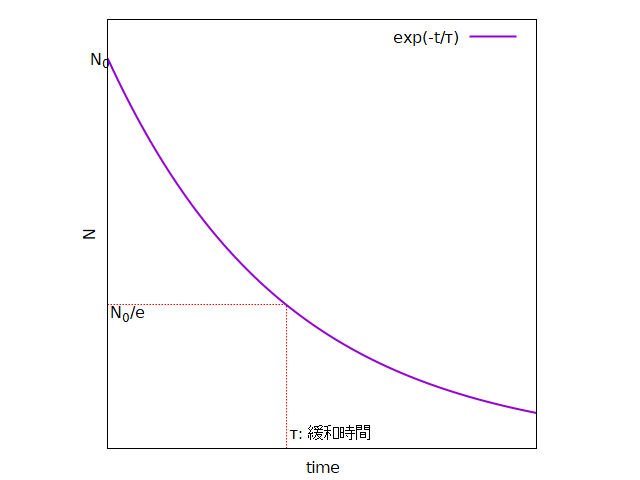
\includegraphics[width=\textwidth]{relux_1.png}
			\end{center}
		\end{minipage}
		\caption{指数関数的減少と緩和時間}
		\label{fig:exp_kanwa}
	\end{center}
\end{figure}

グラフから、時間の次元を持つ $\tau$ は、初期濃度の $\dfrac{1}{e}$ となる時間であることがわかります。
この、指数関数の時間に伴う現象を表す特徴的な時間を「緩和時間\index{かんわじかん@緩和時間}」と呼びます。
\large
	\begin{itembox}[l]{緩和時間とは}
		\begin{itemize}
			\item 時間の次元を持つ $\tau$ は、初期濃度の $\dfrac{1}{e}$ となる時間を表します。
			\item この特徴的な時間を「緩和時間」と呼びます。
		\end{itemize}
	\end{itembox}	
\normalsize

\subsubsection{緩和時間\index{かんわじかん@緩和時間}についてもう少し}

緩和時間\index{かんわじかん@緩和時間}の意味について、もう少し考察をしてみましょう。

濃度変化は以下の式で書けるのでした。
\begin{align*}
	N(t) = N_0 \exp \left(-\dfrac{t}{\tau} \right)
\end{align*}

この濃度の式を時間で微分すると、減少速度は以下の式となります。
\begin{align*}
	\dfrac{\mathrm{d}N(t)}{\mathrm{d}t} = -\dfrac{N_0}{\tau} \exp \left(-\dfrac{t}{\tau} \right)
\end{align*}

したがって、$t=0$ での減少速度は、以下となります。
\begin{align*}
	\dfrac{\mathrm{d}}{\mathrm{d}t}N(0) &=-\dfrac{N_0}{\tau} \exp \left(-\dfrac{0}{\tau} \right) \\
	&=-\dfrac{N_0}{\tau}
\end{align*}

結局、初期状態($t=0$)での減少速度を維持して濃度が減少したとすれば、緩和時間 $\tau$ だけ時間経過したときに濃度が 0 となることになります。
\begin{figure}[htb]
	\begin{center}
		\begin{minipage}{0.45\textwidth}
			\large
			\begin{itembox}[l]{緩和時間のもう一つの意味}
				\begin{itemize}
					\item 初期速度を維持して濃度が\\減少すると、
					\item $t=\tau$ で濃度が 0
				\end{itemize}
			\end{itembox}
		\end{minipage}
		\begin{minipage}{0.45\textwidth}
			\begin{center}
			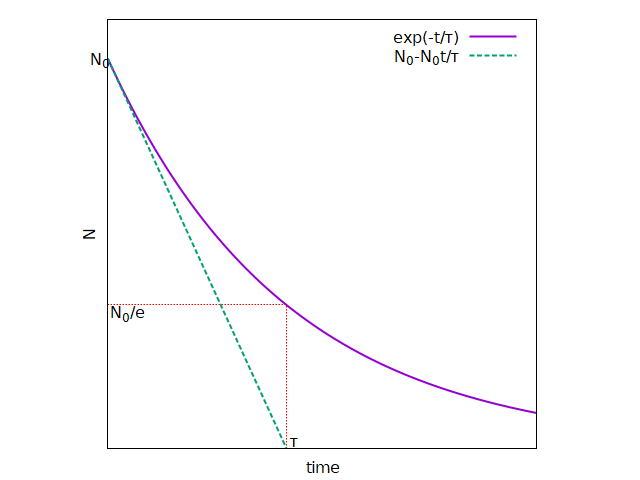
\includegraphics[width=\textwidth]{relux_2.png}
			\end{center}
		\end{minipage}
		\caption{緩和時間のもう一つの意味}
		\label{fig:exp_kanwa2}
	\end{center}
\end{figure}

\section{物理モデルを物質の物理とつなげるために}

ここでは、「物理モデル\index{ぶつりもでる@物理モデル}」として仮想的にイメージできるモデルを実際の物質での物理とつなげていくために、力、仕事、エネルギーという大事な物理量を確認します。
その理解の上で、物質のマクロ及びミクロでの状態を記述するポテンシャルと力の関係が微積分でつながっていることを見て行きます。

\subsection{仕事\index{しごと@仕事}、エネルギー\index{えねるぎー@エネルギー}}

まず、最初に、仕事とエネルギーの確認から始めましょう。

仕事とは、「質点に力\index{ちから@力}を作用して、移動すること」であり、物理量としては、「仕事 $W$ は、作用させた力 $F$ と移動した距離 $s$ の積」として定義されます。
\begin{align*}
	W=F \times s
\end{align*}
\begin{figure}[htb]
	\begin{center}
		\begin{minipage}{0.42\textwidth}
			\large
			\begin{itembox}[l]{仕事とは}
				\begin{itemize}
					\item 質点に力を作用して、移動すること
					\item 仕事は、作用させた力 $F$ と移動した距離 $s$ の積
				\end{itemize}
					
\includegraphics[width=.8\textwidth]{work.png}
			\end{itembox}
		\end{minipage}
		\begin{minipage}{0.42\textwidth}
			\large
			\begin{itembox}[l]{エネルギーとは}
				\begin{itemize}
					\item 仕事をする能力のこと
					\item 物体や空間(場)は、その状態を変えることによりエネルギーを蓄える。
					\item 仕事とエネルギーの次元は同一。
				\end{itemize}
			\end{itembox}
		\end{minipage}
		\caption{仕事とエネルギー}
		\label{fig:work_energy}
	\end{center}
\end{figure}



エネルギー\index{えねるぎー@エネルギー}は、「仕事\index{しごと@仕事}をする能力」のことであり、仕事とエネルギーの次元は同一となっています。
したがって、物体や空間(場)は、力学的な仕事を受けることでその状態を変えることによりエネルギーが高い状態となり、エネルギーを蓄えることになります。
\large
\begin{itembox}[l]{仕事とエネルギーの次元と組み立て単位}
	\begin{itemize}
		\item 次元:[仕事] = [力][距離] = [$ML^2T^{-2}$]
		\item 組み立て単位:ジュール J
	\end{itemize}
\end{itembox}
\normalsize

レオロジーにおいては、外力\index{がいりょく@外力}に対応して物質が変形したとき、静力学的な釣り合いのもとで物質が仕事をされたと考えることができます。
言い換えれば、外力\index{がいりょく@外力}が物質の内部に蓄積された(弾性\index{だんせい@弾性})エネルギーに相当する量の仕事を行ったことになります。

\subsection{ポテンシャル\index{ぽてんしゃる@ポテンシャル}と力\index{ちから@力}と微積分\index{びせきぶん@微積分}}
次に、ポテンシャルについて考えましょう。
\large
\begin{itembox}[l]{ポテンシャルとは?}
	\begin{itemize}
		\item 基準の状態を定めて、
		\begin{itemize}
			\item その着目する状態にするために、
			\item その物体あるいは空間に加えた仕事の量
		\end{itemize}
		\item 逆に言えば
		\begin{itemize}
			\item ある状態から基準の状態に戻るまでに、
			\item 外に取り出すことのできるエネルギーの量
		\end{itemize}
		\item 力が「\textcolor{red}{保存力}」であれば、
		\item ポテンシャルが「位置のみの関数の\textcolor{red}{状態量}」となる
	\end{itemize}
	\begin{screen}
		\begin{itemize}
			\item 保存力\index{ほぞんりょく@保存力}:仕事が経路によらないように定義できる力
			\item 状態量:系の状態だけで、一意に決まる物理量
		\end{itemize}
	\end{screen}
\end{itembox}
\normalsize

ポテンシャル\index{ぽてんしゃる@ポテンシャル}とは、「任意の基準の状態を定めたうえで、着目する状態にするためにその物体あるいは空間に加えた仕事の量」と定義することができます。
このことを逆に言えば、「ある状態から基準の状態に戻るまでに外に取り出すことのできるエネルギー\index{えねるぎー@エネルギー}の量」と考えることもできます。

このとき、対象としている環境の違いが重要となります。
力が「保存力\index{ほぞんりょく@保存力}」であれば、ポテンシャルは「位置のみの関数として与えられる状態量」となるのですが、実際の物質ではそうならない場合もよく生じてしまいます。
このことについては、次の項目で説明します。
\begin{figure}[htb]
	\begin{center}
		\begin{minipage}{0.4\textwidth}
			\large
			\begin{itembox}[l]{ポテンシャル $U(\bm{r})$は、}
				\begin{itemize}
					\item 基準の位置 $\bm{r_0}$ から、
					\item 位置 $\bm{r}$ までの、
					\item 力 $F(\bm{r})$ の積分
				\end{itemize}
				\vspace{-3mm}
				% \small
				\begin{align*}
					W(\bm{r}) = \int_{\bm{r_0}}^{\bm{r}} F(\bm{r}) \rmd \bm{r} = -U(\bm{r})
				\end{align*}
			\end{itembox}
			\begin{itembox}[l]{力 $F(\bm{r})$は、}
				\begin{itemize}
					\item 任意の位置で、
					\item $U(\bm{r})$ を微分すれば、
				\end{itemize}
				\vspace{-3mm}
				% \small
					\begin{align*}
						\dfrac{\mathrm{d}}{\mathrm{d}\bm{r}} U(\bm{r}) = -F(\bm{r})
					\end{align*}
			\end{itembox}
		\end{minipage}
		\begin{minipage}{0.5\textwidth}
			\begin{center}
			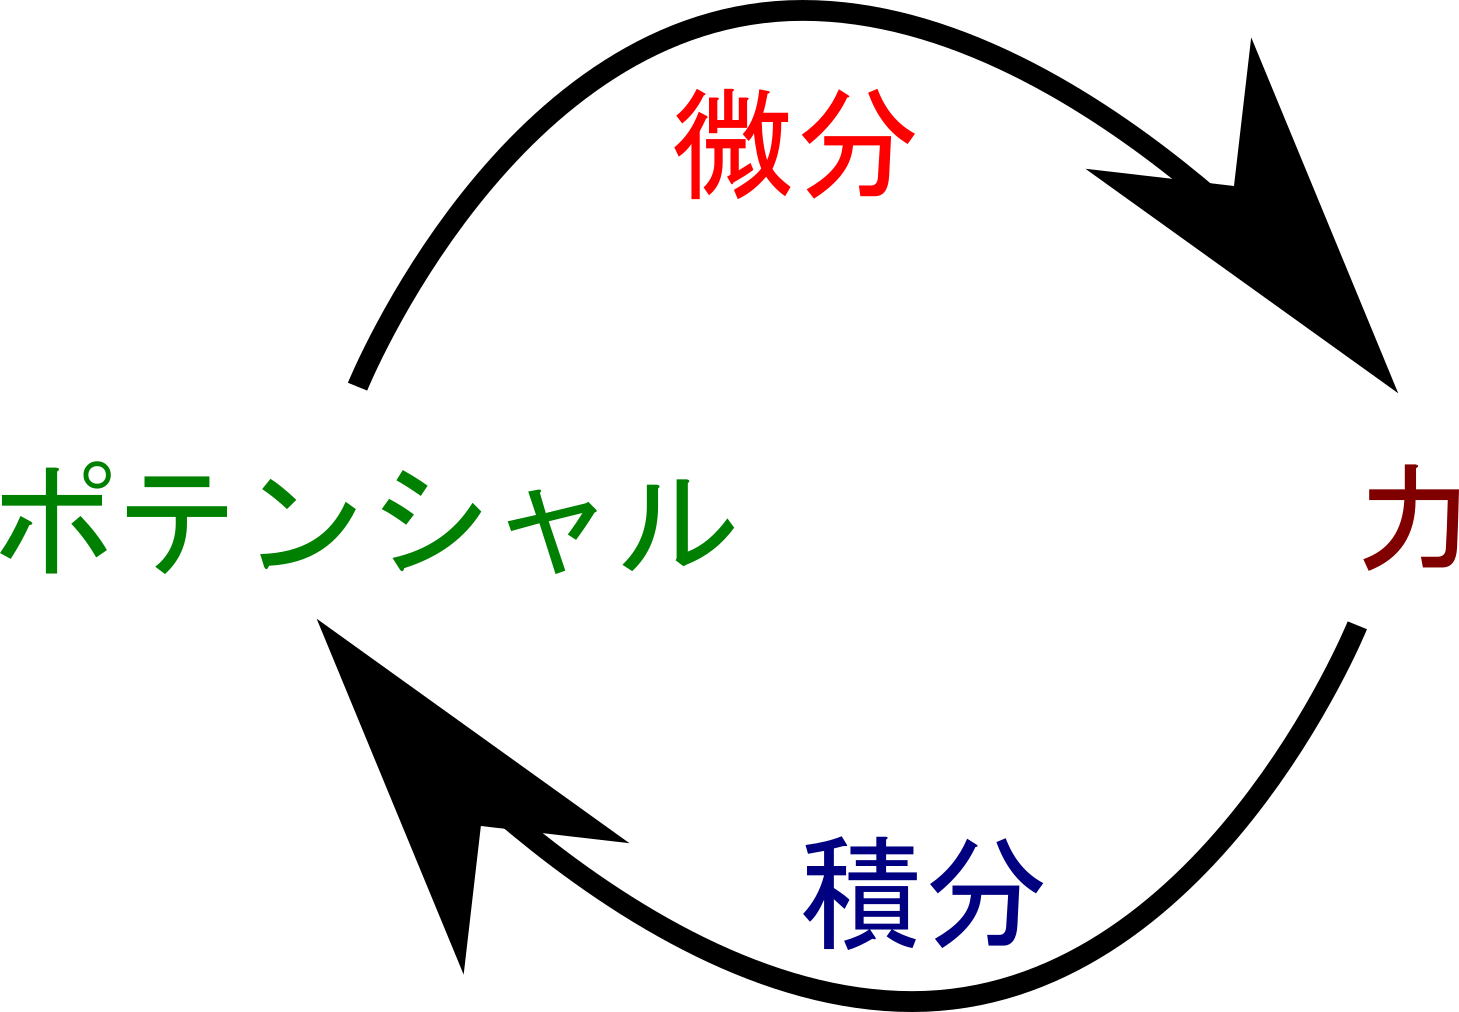
\includegraphics[width=.9\textwidth]{potential_power.png}
			\end{center}
		\end{minipage}
		\caption{ポテンシャルと力と微積分}
		\label{fig:pot_power}
	\end{center}
\end{figure}

力\index{ちから@力}を保存力として考えられる、理想的な状態においてもう少し整理します。

ポテンシャル\index{ぽてんしゃる@ポテンシャル}は、基準の位置 $\bm{r_0}$ から、任意の位置 $\bm{r}$ までの、力 $F(\bm{r})$ の積分として以下のように書けます。

	\begin{align*}
		W(\bm{r}) = \int_{\bm{r_0}}^{\bm{r}} F(\bm{r}) \rmd \bm{r} = -U(\bm{r})
	\end{align*}

逆に言えば、任意の位置でポテンシャル $U(\bm{r})$ を微分すれば、その位置での力を算出することができ、結局、表裏一体の逆変換として捉えることができるわけです。
\begin{align*}
	\dfrac{\mathrm{d}}{\mathrm{d}\bm{r}} U(\bm{r}) = -F(\bm{r})
\end{align*}



\subsection{摩擦力\index{まさつりょく@摩擦力}、非保存力\index{ひほぞんりょく@非保存力}}

この節の最後に、現実の世界に少し近づいてみましょう。

ここまでの議論の大半は、力が保存力であり仕事\index{しごと@仕事}やポテンシャルが状態料として考えられる、高校までの物理で取り扱っていた理想的(仮想的)な状態での議論でした。
実際の我々の周りで生じている事象は、そんなに単純ではなく、ものを移動させようとすると摩擦という抵抗が生じてきます。
\begin{figure}[htb]
	\begin{center}
		\begin{minipage}{0.45\textwidth}
			\large
			\begin{itembox}[l]{摩擦と熱}
				\begin{itemize}
					\item 摩擦力は非保存力
						\begin{itemize}
							\item ポテンシャルは状態量ではなく経路に依存
						\end{itemize}
					\item 内部の粒子の摩擦により、
						\begin{itemize}
							\item 粒子の運動エネルギーが増加し系全体の温度が上昇
							\item 非断熱系では、熱エネルギーとして外界に散逸。
						\end{itemize}
					\item 非保存力も含めれば、系全体のエネルギーは保存
				\end{itemize}
			\end{itembox}
		\end{minipage}
		\begin{minipage}{0.45\textwidth}
			\begin{center}
			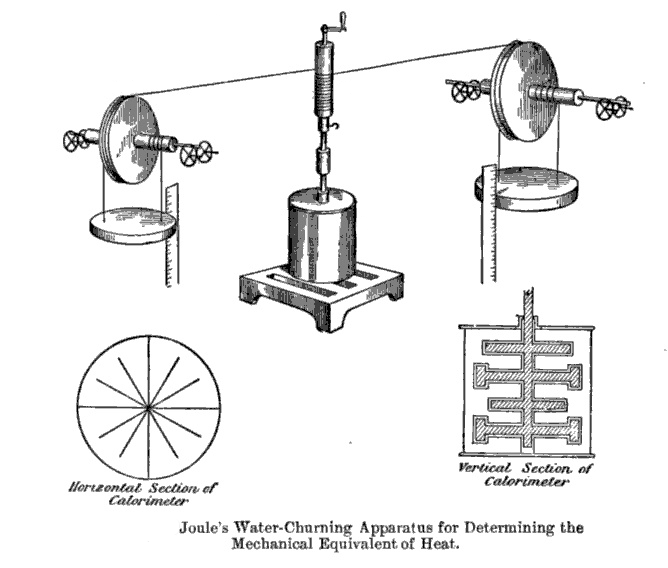
\includegraphics[width=\textwidth]{thermal_eng.png}
			\end{center}
		\end{minipage}
		\caption{摩擦力、熱}
		\label{fig:masatsu_netsu}
	\end{center}
\end{figure}

摩擦力は非保存力であり、摩擦を考慮した系においては、ポテンシャルは状態量ではなく経路に依存することになります。
摩擦が生じる原因については、これも細かく考えていくとややこしくなってきますので、ここでは現実に生じているものだということで詳細には立ち入りません。

ただ、レオロジー的に考えるときに、次の章で議論するような内部の粒子\index{りゅうし@粒子}を想定してモデルを設定すると、粒子同士の摩擦により、粒子\index{りゅうし@粒子}の運動エネルギー\index{ねつえねるぎー@運動エネルギー}が増加し系全体の温度が上昇するという状態をイメージすることができます。
このようにして発生した熱が、断熱していない系では、熱エネルギー\index{ねつえねるぎー@熱エネルギー}として外界に散逸することになります。

このような非保存力も含めて考えれば、系全体のエネルギーは保存することになります。
図 \ref{fig:masatsu_netsu} には、保温した容器の中の水を撹拌することにより、熱が仕事と等価であることを示したジュールの実験装置の概略を示しました。

\section*{この章のまとめ}

この章では、具体的なレオロジーの議論に入る前に、これからの議論に必要となる数学と物理の基礎的な事項について、高校から大学レベルの内容を確認しました。
\begin{boxnote}
	\large
	\begin{itemize}
		\item 数学的な事項について
			\begin{itemize}
				\item レオロジーで扱う関数について、指数関数とその逆関数に対応する対数関数の確認
				\item 微積分について、微分が「瞬間的な振る舞いを記述」し、積分が「全体の量を把握」する
				\item 簡単な微分方程式をとくことで、レオロジー関連の事項で頻出の「指数関数的な応答」を理解
			\end{itemize}
		\item 物理に関する事項として
			\begin{itemize}
				\item 次元について、「次元解析」や「無次元量」について
				\item 力、仕事、ポテンシャルを確認して、その微積分との関係について
			\end{itemize}
	\end{itemize}
\end{boxnote}

\newpage

\begin{longartdeco}
	\begin{center}
	\emph{コラム:「褒めて育てる」?}	
	\end{center}

	著者は、「地声も大きく、気も短くて、かつ、物事を曖昧にしておくのが苦手」なので、つい、いろんなことを確認のつもりでポンポンと根掘り葉掘り聞いてしまいます。
	この態度が、年下の人に対する圧迫的な振る舞いに見えるようで、あなたはパワハラ体質ですねとよく指摘されてしまいます。
	「叱って指導しても人は育ちません」と諭されてしまうことも度々でした。
	
	「部下は褒めて育てる。」ということが、最近のトレンドになっています。
	確かに、人は叱られるよりは褒められたほうが気持ちがいいので、「北風よりは太陽」を好みます。
	そのような環境のほうがのびのびと仕事が進むはずでしょう。
	
	でも、この「褒めるマネージメント」が、いつもうまくいくかというとそういうわけでもないようです。
	例えば、部下の方が褒められそうな行動を前もって予測して、そのような行動だけを取るようになってしまう場合もよく見かけます。
	その結果として、上司の耳あたりの良いことだけを選んで報告して都合の悪いことは無視(隠して)してしまうこともあります。
	これでは、自主性もなく、上司の気持ちだけを「忖度する部下」を養成しているのかもしれません。
	一見できる部下という、ちょっと世渡りの下手な(出来の悪いとされがちな)人よりもたちの悪い、本当に困った部下を作り出す環境なのかもしれません。
	
	ということで、どちらの方法でも、うまく行かないことが多いわけです。
	見方を変えてみると、叱るにしても、褒めるにしても、上司(あなた)の主観、判断、都合が入っているわけです。
	では、どうすればいいのでしょうか?
	
	この境目が、「きちんと承認する」ということになるのかもしれません。
	きちんと目の前にある事実から目をそらすことなく、自身の思い込みだけに頼ることなく、あるがままの状態を一旦そのままで受け入れてから、
	その「あるべき状態を想像しながら対応する。」という態度が、一番公平な対応ではないでしょうか。
	
	これって、結局、(中立的に)科学的な態度で目の前の事象に対応するということになるわけです。
	そのうえで、コミュニケーションの基本である「相手に自身の認識を正しく伝える」ということを愚直に行えばいいのでしょう。
	この対応が、上記の「きちんと承認する」という行為になるので、中立的な表現として受け手(部下)にシンプルに伝わることが期待できます。
	
	ということで、「科学的なアプローチをきちんと行った上で、コミュニケーション能力の向上に少しだけ努力するというあたりが一番妥当な道かな?」と思う今日この頃です。


\end{longartdeco}


\end{document}